\section{\hfil Lab Worksheet IV \hfil}
\subsection*{Univariate analysis and graphing}
\addcontentsline{toc}{subsection}{Univariate analysis and graphing}

Today we are going to use data from the ESS 2012 again. You can find the dataset on LEARN; make sure you download \textbf{essuk12v2.dta} (notice the ``v2''). In this lab session we are going to do some basic descriptive statistics, including tabulating and graphing. One of the simplest things in data analysis is reporting descriptive statistics and simple graphs that show a single variable. This is what we call \textbf{univariate analysis}, and it is very useful when trying to summarise and describe data (which in in turn helps finding patterns in the data). In Stata there are multiple ways to look at descriptive statistics. Last week you were introduced to two useful commands: \texttt{describe} and \texttt{codebook}. Today you will use one more: \texttt{summarize}. Let’s take a look at it, try typing

\begin{lstlisting}
	summarize
\end{lstlisting} 

and you will see a list of summary statistics for all the variables present in your dataset. This command can be shortened to \texttt{su}, and it allows for a selection of variables like this:

\begin{lstlisting}
	su gender tvtot
\end{lstlisting}

In the example above the command \texttt{summarize} only reports on two variables (``gender'' and ``tvtot''). Notice that the command is \texttt{summarize} and not \texttt{summarise}. This command, as you can see, tells you the number of observations, the mean of the variable, the standard deviation, and the minimum and maximum values a variables takes on. Let's now revise the command \texttt{codebook} with an extra option (remember that \texttt{codebook} cannot be shortened):

\begin{lstlisting}
	codebook gender tvtot, compact
\end{lstlisting}

As you can see, \texttt{codebook, compact} provides you with similar information (but not the same). In this case you get variable labels and unique values. Also notice that the command option follows a comma, which tells Stata that you have decided to use an option. You can try typing the following to see what the option \texttt{compact} really does:

\begin{lstlisting}
	codebook gender tvtot
\end{lstlisting}

The option \texttt{compact} presents you with a shorter report, which you might want if presenting summary statistics to someone else. Remember that you also have the \texttt{describe} command:

\begin{lstlisting}
	de gender tvtot
\end{lstlisting}

Just like the other two commands, you can use \texttt{describe} on the entire dataset or on a selection of variables. The important thing to notice is that these three commands report similar yet different information. Now give these commands a try and find the following information:

\begin{itemize}
	\item The variable labels for all variables in the dataset.
	\item The mean of the variable ``age.''
	\item The mode of the variable ``tvtot.''
	\item The minimum and the maximum values of the variable ``socmeet.''
\end{itemize}

After completing the exercise above you might have noticed that the maximum value of ``socmeet'' is oddly high. The answer has to do with response categories. For example, the ESS codes ``Don't know'' as ``88'' and ``Not available'' as ``999.'' This coding allows you identify these categories easily across variables and treat them as \textbf{missing data}. Different datasets will code these categories in different ways, but it is important to know how these categories are coded before doing data analysis.

\subsection*{Tabulating data}

The command \texttt{tabulate}, which you can shorten to \texttt{tab}, creates one-way or two-way tables of frequencies. The command is followed by one or two variables of your interest, for instance:

\begin{lstlisting}
	tabulate socmeet
\end{lstlisting}

If you were interested in seeing the codes of the response categories you could add a command option to \texttt{tabulate} like in the example below (remember that command options follow a comma):

\begin{lstlisting}
	tab socmeet, nolabel
\end{lstlisting}

The option \texttt{nolabel} removes value labels from the tabulation, and it can be shortened to \texttt{nol}. This option could be useful to see at a glance how a variable is coded (but remember that \texttt{codebook} also shows you this information). Now let's change ``Don't know'' to something else that Stata understands as \textbf{missing values}. The command \texttt{replace} will be handy here:

\begin{lstlisting}
	replace socmeet=.a if socmeet==88
\end{lstlisting}

As you can imagine, \texttt{replace} replaces the content of an existing variable, in this case ``socmeet.'' Notice that in the command above there is an \texttt{if} qualifier. This qualifier is telling Stata to perform an action only on those cases that meet the qualification, which in this case is ``when the variable ``socmeet'' equals 88.'' In other words, the command above is saying something like ``for those observations in which the variable ``socmeet'' is ``88'', replace ``socmeet's'' value ``88'' to ``.a''. The baseline dot before the ``a'' is of paramount importance because that is how Stata recognises missing values. Also notice that Stata distinguishes between ``='' and ``=='' (like many other programming languages). The former (``='') is used as a set equal operator, whereas the latter (``=='') is used to test for equality. You can find more about this topic in the ``Stata Cheatsheet'' on LEARN. Now that you have coded the missing values in the variable ``socmeet'' let's tabulate it again:

\begin{lstlisting}
	tab socmeet
\end{lstlisting}

If you compare this new tabulation to the first one, you will notice that three cases are now missing (i.e., the three cases who responded ``Don't know''). You can check how many missing cases a variable has using the \texttt{missing} option like this:

\begin{lstlisting}
	tab socmeet, missing
\end{lstlisting}  

\forceindent \textbf{?} Now try all this by yourself. Let's look for missing values in the variables ``age'', ``gender'', and ``houseincome.'' If you find missing values change them to something like ``.a'' or ``.b''. Do not forget to use command options like \texttt{nolabel} and \texttt{missing}.

The \texttt{if} qualifier can also be used in the command \texttt{tabulate}. For example, say you want to tabulate the gender of those respondents older than 30:

\begin{lstlisting}
	tab gender if age > 30
\end{lstlisting}
 
 Notice that the variable-target of \texttt{tabulate} is ``gender'' whereas the target of the qualifier \texttt{if} is ``age.'' You can be even more specific with your tabulations, for example:
 
\begin{lstlisting}
	tab gender if age > 30 & age < 50
\end{lstlisting}

Notice that after \texttt{\&} (``and'') you need to specify again the target-variable (in this case ``age''). You can use as many variables as you want. Say you wish to know the gender distribution of those of 20 years of age \textbf{or more} and who voted in the last national election:

\begin{lstlisting}
	tab gender if vote==1 & age >= 20
\end{lstlisting}

\forceindent \textbf{?} Try now to find out how many observations are below the fifth decile in the variable ``hoseincome.''

\subsection*{Graphing data}

Producing graphs is an extremely powerful (and useful) way of examining your data. Stata allows you to produce a great variety of graphs, as well as it allows you to customise them. Let's start by producing a pie chart of the average number of hours watching TV (variable ``tvtot''). Using the menu, go to \textbf{Graphics > Pie chart}. Make sure \textit{Graph by categories} is selected, and where it says \textit{Category variable} select ``tvtot.'' Now click on \textbf{Submit} and you will get a pie chart of the variable ``tvtot.'' In your results-window you can see the command for this action:

\begin{lstlisting}
 graph pie, over(tvtot)
\end{lstlisting}

Let's make the plot a bit more attractive. Go to the \textbf{Slices} tab and select \textit{Customize all slice properties}. Then click on \textit{Slice properties (all)}, tick \textit{Explode slide} and in the drop-down menu select \textit{Automatic}. In the same window, select \textit{Customize all slice labels} and click on \textit{Label properties (all)}. In \textit{Label type} select \textit{Percent}. Now click on \textit{OK} and submit your graph. Stata reports the command for all this clicking and pointing in the results-window. You can use that command to reproduce the exact same graph granted that the variable ``tvtot'' remains the same.

\begin{figure}[H]
	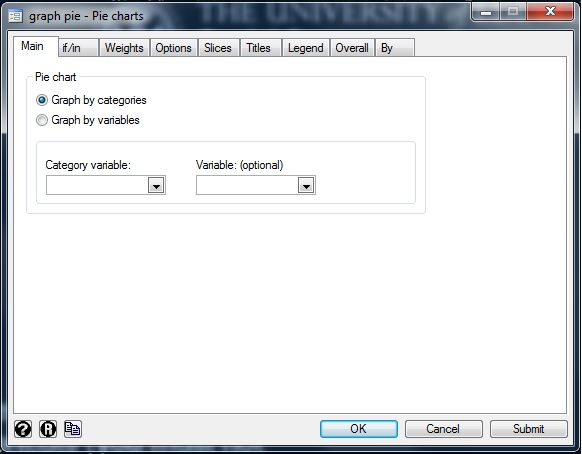
\includegraphics[width=\linewidth]{./img/graphics_pie.jpg}
	\caption{Stata's Graphics > Pie chart.}
\end{figure}
